\newpage
\subsection{\MsPacManName}

Two clusterings are examined for \MsPacManName (Table~\ref{tab:qualitative_ms_pacman_metrics}), obtained at layer 6b with $K=3$ and at layer 4 with $K=5$.

With $K=3$ (Figure~\ref{fig:qualitative_ms_pacman}), the partition captures the progress and state of the game rather than a specific spatial feature of the observation.
The start of the episode is captured in cluster B.
The middle of the episode is captured in cluster A.
The end of the episode is captured in cluster C.

With $K=5$ (Figure~\ref{fig:qualitative_ms_pacman_alt}), the partition provides a more detailed description of the episode.
The initial animation, during which the character cannot move, is isolated in cluster H.
The beginning of actual play is captured in cluster F.
A situation specific to the game mechanics, in which Pac-Man is in booster mode and waits in front of the ghost spawn to eat the ghosts, is isolated in cluster D.
The end of the episode, when at most one power pellet remains, is separated into two similar clusters, E and G.

The two clusterings have the same \gls{cu} of $0.88$.
The clustering at layer 4 has a lower \gls{as} of $0.47$ compared with $0.52$ at layer 6b.
This results in a lower \gls{acu} of $0.35$ compared with $0.40$.

\vfill
\begin{table}[H]
    \centering
    \begin{tblr}{
        width=\linewidth,
        colspec={Q[c,wd=1.6cm] X[l]},
        cells = {valign=m},
        rowsep=2pt,
        hline{1,Z} = {1pt},
        hline{5} = {0.5pt},
        hline{2,6} = {0.3pt},
        row{1,5} = {bg=black!8, font=\bfseries},
        column{1} = {font=\bfseries}
    }
        \SetCell[c=2]{l} \makebox[1.9cm][l]{Layer 6b}\makebox[1.4cm][l]{$K=3$}\makebox[2.75cm][l]{\gls{cu} 0.88}\makebox[2.75cm][l]{\gls{as} 0.52}\gls{acu} 0.40 & \\
        A & Middle of the episode. \\
        B & Start of the episode. \\
        C & End of the episode. \\
        \SetCell[c=2]{l} \makebox[1.9cm][l]{Layer 4}\makebox[1.4cm][l]{$K=5$}\makebox[2.75cm][l]{\gls{cu} 0.88}\makebox[2.75cm][l]{\gls{as} 0.47}\gls{acu} 0.35 & \\
        D & Pac-Man is in booster mode and waits in front of the ghost spawn to eat the ghosts. \\
        E & End of the episode, at most one power pellet remains (similar to cluster G). \\
        F & Start of the episode. \\
        G & End of the episode, at most one power pellet remains (similar to cluster E). \\
        H & Start-of-episode animation, the character cannot move. \\
    \end{tblr}
    \caption{\gls{cu}, \gls{as}, and \gls{acu} of the two clusterings analyzed in the \MsPacManName environment.}
    \label{tab:qualitative_ms_pacman_metrics}
\end{table}
\vfill

\newpage
\vspace*{\fill}
\begin{figure}[t]
    \centering
    \resizebox{\textwidth}{!}{
    \begin{tikzpicture}

    \node (ligne_1) at (0, 0) {};

    \node[] at ($(ligne_1) + (-4.5cm, 0cm)$) {
    \begin{minipage}{4.5cm}
        \centering
        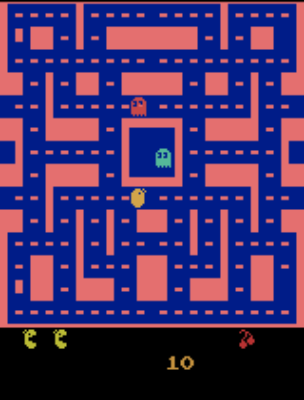
\includegraphics[width=2cm]{figures/clustering_agent_representation/pictures/ms_pacman/qualitative/cluster_1/image_1.png}
        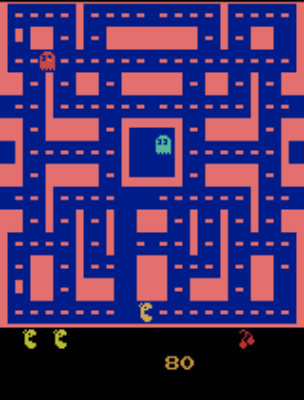
\includegraphics[width=2cm]{figures/clustering_agent_representation/pictures/ms_pacman/qualitative/cluster_1/image_2.png}

        \small Start of the episode.
    \end{minipage}
    };

    \node[] at ($(ligne_1) + (0cm, 0cm)$) {
    \begin{minipage}{4.5cm}
        \centering
        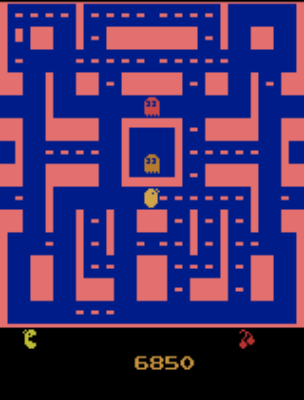
\includegraphics[width=2cm]{figures/clustering_agent_representation/pictures/ms_pacman/qualitative/cluster_0/image_1.png}
        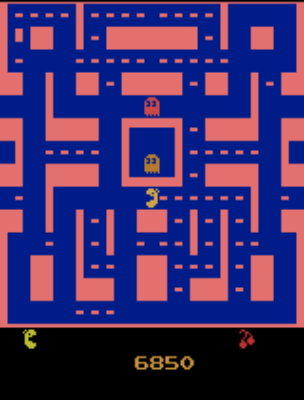
\includegraphics[width=2cm]{figures/clustering_agent_representation/pictures/ms_pacman/qualitative/cluster_0/image_2.png}

        \small Middle of the episode.
    \end{minipage}
    };

    \node[] at ($(ligne_1) + (4.5cm, 0cm)$) {
    \begin{minipage}{4.5cm}
        \centering
        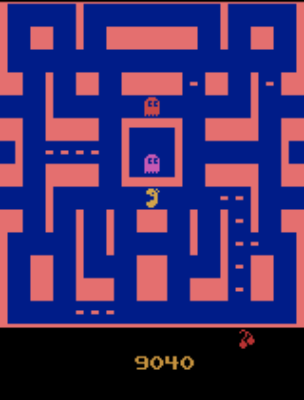
\includegraphics[width=2cm]{figures/clustering_agent_representation/pictures/ms_pacman/qualitative/cluster_2/image_1.png}
        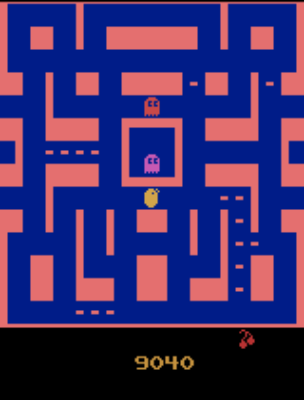
\includegraphics[width=2cm]{figures/clustering_agent_representation/pictures/ms_pacman/qualitative/cluster_2/image_2.png}

        \small End of the episode.
    \end{minipage}
    };

    \end{tikzpicture}
    }
    \caption{Clusters identified by \gls{car} in the Ms.\ Pac-Man environment (layer 6b, $K=3$).}
    \label{fig:qualitative_ms_pacman}
\end{figure}


\begin{figure}[H]
    \qualitativeClusterFigureSetup
    \qualitativeClusterTwo
        {figures/clustering_agent_representation/pictures/ms_pacman/qualitative_alt/cluster_0/image_1.png}
        {figures/clustering_agent_representation/pictures/ms_pacman/qualitative_alt/cluster_0/image_2.png}
        {D}
    \qualitativeClusterTwo
        {figures/clustering_agent_representation/pictures/ms_pacman/qualitative_alt/cluster_1/image_1.png}
        {figures/clustering_agent_representation/pictures/ms_pacman/qualitative_alt/cluster_1/image_2.png}
        {E}
    \qualitativeClusterTwo
        {figures/clustering_agent_representation/pictures/ms_pacman/qualitative_alt/cluster_2/image_1.png}
        {figures/clustering_agent_representation/pictures/ms_pacman/qualitative_alt/cluster_2/image_2.png}
        {F}
    \qualitativeClusterTwo
        {figures/clustering_agent_representation/pictures/ms_pacman/qualitative_alt/cluster_3/image_1.png}
        {figures/clustering_agent_representation/pictures/ms_pacman/qualitative_alt/cluster_3/image_2.png}
        {G}
    \qualitativeClusterTwo
        {figures/clustering_agent_representation/pictures/ms_pacman/qualitative_alt/cluster_4/image_1.png}
        {figures/clustering_agent_representation/pictures/ms_pacman/qualitative_alt/cluster_4/image_2.png}
        {H}
    \caption{Clusters D--H identified by \gls{car} in the \MsPacManName environment (layer 4, $K=5$).}
    \label{fig:qualitative_ms_pacman_alt}
\end{figure}

\vfill
